\section{Evaluation}
\label{sprout:eval}

This section presents our experimental results obtained using the
testbed described
in \S\ref{ss:platform}. We start by motivating and defining the two
main metrics: throughput and self-inflicted delay. We then compare
Sprout with Skype, Facetime, and Hangouts, focusing on how the
different rate control algorithms used by these systems affect the
metrics of interest. We compare against the delay-triggered congestion
control algorithms TCP Vegas and LEDBAT, as well as the
default TCP in Linux, Cubic, which does not use delay as a
congestion signal, and Compound TCP, the default in some
versions of Windows.

We also evaluate a simplified version of Sprout, called Sprout-EWMA,
that eliminates the cautious packet-delivery forecast in favor of an
exponentially-weighted moving average of observed throughput. We
compare both versions of Sprout with a queue-management technique that
must be deployed on network infrastructure. We also measure Sprout's
performance in the presence of packet loss.

Finally, we evaluate the performance of competing flows (TCP Cubic
and Skype) running over the Verizon LTE downlink, with and without
SproutTunnel.

The implementation of Sprout (including the tuning parameters $\sigma
= 200$ and $\lambda_z = 1$) was frozen before collecting the network
traces, and has not been tweaked.
% However, SproutTunnel and its AQM
%scheme were designed and evaluated after the network traces were
%collected and the rest of the evaluation had been conducted.

\subsection{Metrics}

We are interested in performance metrics appropriate for a real-time
interactive application. In our evaluation, we report the
\emph{average throughput} achieved and the 95th-percentile
\emph{self-inflicted delay} incurred by each protocol, based on
measurement of packet entry and exit from the Cellsim.

The \emph{throughput} is the total number of bits received by an
application, divided by the duration of the experiment. We use this as
a measure of bulk transfer rate.

The {\em self-inflicted delay} is a lower bound on the end-to-end
delay that must be experienced between a sender and receiver, given
observed network behavior. We define it as follows: At any point in
time, we find the most recently sent packet to have arrived at the
receiver. The amount of time since this packet was sent is a lower
bound on the instantaneous delay that must exist between the sender's
input and receiver's output in order to avoid a gap in playback or
other glitch at this moment. We calculate this instantaneous delay for
each moment in time. The 95th percentile of this function (taken over the
entire trace) is the amount of delay that must exist between the input
and output so that the receiver can recover 95\%~of the input signal
by the time of playback. We refer to this as ``95\%~end-to-end
delay.''

For a given trace, there is a lower limit on the 95\%~end-to-end delay
that can be achieved even by an omniscient protocol: one that sends
packets timed to arrive exactly when the network is ready to dequeue
and transmit a packet. This protocol will achieve
100\%~of the available throughput of the link and its packets will
never sit in a queue. Even so, the omniscient protocol will have
fluctuations in its 95\%~end-to-end delay, because the link may have
delivery outages. If the link does not deliver any packets for 5
seconds, there must be at least 5 seconds of end-to-end delay to avoid
a glitch, no matter how smart the protocol is.\footnote{If packets are
  not reordered by the network, the definition becomes simpler. At
  each instant that a packet arrives, the end-to-end delay is equal to
  the delay experienced by that packet. Starting from this value, the
  end-to-end delay increases linearly at a rate of 1 s/s, until the
  next packet arrives. The 95th percentile of this function is the
  95\%~end-to-end delay.}

The difference between the 95\%~end-to-end delay measured for a
particular protocol and for an omniscient one is known as the
\emph{self-inflicted delay}. This is the appropriate figure to assess
a real-time interactive protocol's ability to compromise between
throughput and the delay experienced by users.

To reduce startup effects when measuring the average throughput and
self-inflicted delay from an application, we skip the first minute of
each application's run.

\subsection{Comparative performance}

\begin{figure*}
\caption{Throughput and delay of each protocol over the traced
  cellular links. Better results are up and to the right.}

\vspace{\baselineskip}
\begin{centering}
\noindent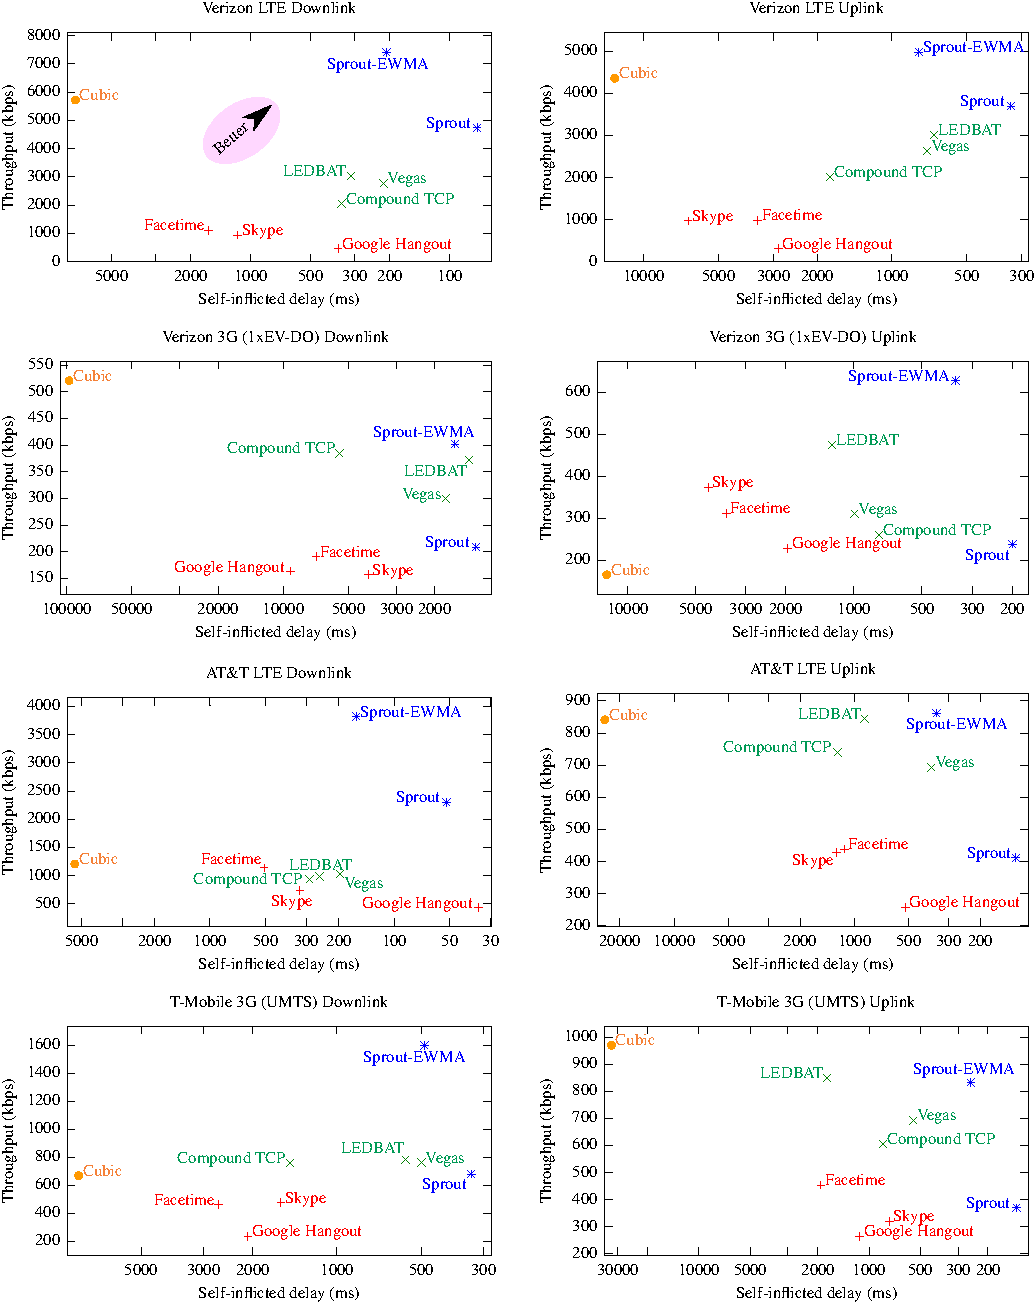
\includegraphics[width=\textwidth]{graphs-out.pdf}

\end{centering}

\label{f:allgraphs}

\end{figure*}

Figure~\ref{f:allgraphs} presents the results of our trace-driven
experiments for each transport protocol. The figure shows eight
charts, one for each of the four measured networks, and for each data
transfer direction (downlink and uplink). On each chart, we plot one
point per application or protocol, corresponding to its measured
throughput and self-inflicted delay combination. For interactive
applications, high throughput and low delay (up and to the right) are
the desirable properties. The table in the introduction shows the
average of these results, taken over all the measured networks and
directions, in terms of the average relative throughput gain and delay
reduction achieved by Sprout.

We found that Sprout had the lowest, or close to the lowest, delay
across each of the eight links. On average delay, Sprout was lower
than every other protocol. On average throughput, Sprout outperformed
every other protocol except for Sprout-EWMA and TCP Cubic.

We also observe that Skype, Facetime, and Google Hangouts all have
lower throughput and higher delay than the TCP congestion-control
algorithms. We believe this is because they do not react to rate
increases and decreases quickly enough, perhaps because they are
unable to change the encoding rapidly, or unwilling for perceptual
reasons.\footnote{We found that the complexity of the video signal did
  not seem to affect these programs' transmitted throughputs. On fast
  network paths, Skype uses up to 5 Mbps even when the image is
  static.} By continuing to send when the network has dramatically
slowed, these programs induce high delays that destroy interactivity.

\subsection{Benefits of forecasting}

Sprout differs from the other approaches in two significant ways:
first, it uses the packet arrival process at the receiver as the
``signal'' for its control algorithm (as opposed to one-way delays as
in LEDBAT or packet losses or round-trip delays in other protocols),
and second, it models the arrivals as a flicker-noise process to
perform Bayesian inference on the underlying rate. A natural question
that arises is what the benefits of Sprout's forecasting are. To
answer this question, we developed a simple variant of Sprout, which
we call {\em Sprout-EWMA}. Sprout-EWMA uses the packet arrival times,
but rather than do any inference with that data, simply passes them
through an exponentially-weighted moving average (EWMA) to produce an
evolving smoothed rate estimate. Instead of a cautious
``95\%-certain'' forecast, Sprout-EWMA simply predicts that the link will
continue at that speed for the next eight ticks. The rest of the
protocol is the same as Sprout.

The Sprout-EWMA results in the eight charts in Figure~\ref{f:allgraphs}
show how this protocol performs. First, it out-performs all the
methods in throughput, including recent TCPs such as Compound TCP and
Cubic. These results also highlight the role of cautious forecasting:
the self-inflicted delay is significantly lower for Sprout compared
with Sprout-EWMA. TCP Vegas also achieves lower delay on average than
Sprout-EWMA. The reason is that an EWMA is a low-pass filter, which
does not immediately respond to sudden rate reductions or outages (the
tails seen in Figure~\ref{f:vzinter}). Though these occur with low
probability, when they do occur, queues build up and take a
significant amount of time to dissipate.  Sprout's forecasts provide a
conservative trade-off between throughput and delay: keeping delays
low, but missing legitimate opportunities to send
packets, preferring to avoid the risk of filling up queues. Because
the resulting throughput is relatively high, we believe it is a good
choice for interactive applications. An application that is interested
only in high throughput with less of an emphasis on low delay may prefer
Sprout-EWMA.

\subsection{Comparison with in-network changes}

We compared Sprout's end-to-end inference approach against an
in-network deployment of active queue management. We added the CoDel
AQM algorithm~\cite{CoDel} to Cellsim's uplink and downlink queue, to
simulate what would happen if a cellular carrier installed this
algorithm inside its base stations and in the baseband modems or
radio-interface drivers on a cellular phone.

The average results are shown in Figure~\ref{f:codelchart}. Averaged
across the eight cellular links, CoDel dramatically reduces the delay
incurred by Cubic, at little cost to throughput.

Although it is purely end-to-end, Sprout's delays are even lower than
Cubic-over-CoDel. However, this comes at a cost to
throughput. (Numerical results are given in Figure~\ref{f:sproutvsaqm}.)
Sprout-EWMA achieves within 6\% of the same delay as Cubic-over-CoDel,
with 30\% more throughput.

Rather than embed a single throughput-delay tradeoff into the network
(e.g.~by installing CoDel on carrier infrastructure), we believe it
makes architectural sense to provide endpoints and applications with
such control when possible. Users should be able to decide which
throughput-delay compromise they prefer. In this setting, it appears
achievable to match or even exceed CoDel's performance without
modifying gateways.

\begin{figure}
\caption{Average utilization and delay of each scheme. Utilization is
  the average fraction of the cellular link's maximum capacity that
  the scheme achieved.}

\vspace{\baselineskip}

%\footnotesize
\def\svgwidth{\columnwidth}\input{codelcomp.pdf_tex}

\label{f:codelchart}

\end{figure}

\begin{figure}
\caption{Lowering the forecast's confidence parameter allows greater
  throughput at the cost of more delay. Results on the T-Mobile 3G (UMTS)
  uplink:}

\vspace{\baselineskip}

%\footnotesize
\def\svgwidth{\columnwidth}\input{varySprout2.pdf_tex}

\label{f:varysprout}

\end{figure}

\subsection{Effect of confidence parameter}

The Sprout receiver makes forecasts of a lower bound on how many
packets will be delivered with at least 95\% probability. We explored
the effect of lowering this confidence parameter to express a greater
willingness that packets be queued for longer than the sender's 100~ms
tolerance.

Results on one network path are shown in
Figure~\ref{f:varysprout}. The different confidence parameters trace
out a curve of achievable throughput-delay tradeoffs. As expected,
decreasing the amount of caution in the forecast allows the sender to
achieve greater throughput, but at the cost of more delay.
Interestingly, although Sprout achieves higher throughput and lower
delay than Sprout-EWMA by varying the confidence parameter, it never
achieves both at the same time. Why this is---and whether Sprout's
stochastic model can be further improved to beat Sprout-EWMA
simultaneously on both metrics---will need to be the subject of
further study.

\subsection{Loss resilience}
\label{ss:loss}

The cellular networks we experimented with all exhibited low packet
loss rates, but that will not be true in general. To investigate the
loss resilience of Sprout, we used the traces collected from one
network (Verizon LTE) and simulated Bernoulli packet losses
(tail drop) with two different packet loss probabilities, 5\% and 10\%
(in each direction). The results are shown in the table below:
\begin{center}
\small
\begin{tabular}{|l|c|c|}
\hline
 Protocol & Throughput (kbps) & Delay (ms) \\
\hline
\hline
\multicolumn{3}{|c|}{\bf Downlink} \\
\hline
Sprout & 4741 & 73 \\
Sprout-5\% & 3971 & 60 \\
Sprout-10\% & 2768 & 58\\
\hline
\multicolumn{3}{|c|}{\bf Uplink} \\
\hline
Sprout & 3703 & 332 \\
Sprout-5\% & 2598 & 378 \\
Sprout-10\% & 1163 & 314\\
\hline
\end{tabular}
\end{center}

As expected, the throughput does diminish in the face of packet loss,
but Sprout continues to provide good throughput even at high loss
rates. (TCP, which interprets loss as a congestion signal, generally
suffers unacceptable slowdowns in the face of 10\% each-way packet
loss.) These results demonstrate that Sprout is relatively resilient to
packet loss.

\subsection{Sprout as a tunnel for competing traffic}

We tested whether SproutTunnel, used as a tunnel over the
cellular link to a well-connected relay, can successfully isolate
bulk-transfer downloads from interactive applications.

We ran two flows: a TCP Cubic bulk transfer (download only) and a
two-way Skype videoconference, using the Linux version of Skype.

We compared the situation of these two flows running directly over the
emulated Verizon LTE link, versus running them through SproutTunnel
over the same link. The experiments lasted about ten minutes
each.\footnote{In each run, Skype ended the video portion of the call
  once and was restarted manually.}

\begin{center}
{
\small
\noindent \begin{tabular}{|l|l|l|l|}
\hline
& Direct & via Sprout & Change \\
\hline
\hline
Cubic throughput & 8336 kbps & 3776 kbps & \cellcolor{red!20}$-55\%$ \\
Skype throughput & 78 kbps & 490 kbps & \cellcolor{blue!20}$+528\%$ \\
Skype 95\% delay & 6.0~s & 0.17~s & \cellcolor{blue!20}$-97\%$ \\
\hline
\end{tabular}
}
\end{center}

The results suggest that interactive applications can be greatly aided
by running their traffic---and any concurrent bulk transfers---through
Sprout. Without Sprout to mediate, Cubic squeezes out Skype and builds
up huge delays. However, Sprout's conservatism about delay
substantially reduces Cubic's throughput.

\vspace{\baselineskip}

%\end{center}

% \subsubsection{Skype}
% \subsubsection{Facetime}
% \subsubsection{Hangouts}

% \subsection{Comparisons to congestion control algorithms}

% \subsubsection{TCP CUBIC}

% \subsubsection{Compound TCP}

% \subsubsection{TCP Vegas}

% \subsubsection{TCP CUBIC + Codel}

% \subsubsection{LEDBAT}
